\section{ Présentation de l'entreprise}

Natixis est la banque de financement, de gestion, d’assurance et de services financiers du Groupe BPCE, deuxième acteur bancaire en France avec 36 millions de clients à travers ses deux réseaux, Banque Populaire et Caisse d’Epargne.

Avec plus de 16 000 collaborateurs, Natixis intervient dans trois domaines d’activités au sein desquels elle dispose d’expertises métiers fortes : la Banque de Grande Clientèle, l’Épargne & l’Assurance et les Services Financiers Spécialisés.

Elle accompagne de manière durable, dans le monde entier, sa propre clientèle d’entreprises, d'institutions financières et d'investisseurs institutionnels et la clientèle de particuliers, professionnels et PME des deux réseaux du Groupe BPCE. 
%%\begin{figure}[!ht]
   % \center
  %  
\includegraphics[]{./images/natixis.png}
 %   \caption{Image Natixis}   
%\end{figure}
\subsection{Présentation de la  DSI-GM-Global Markets-Distribution}
\section {Description de la mission de stage}
\section {Le stage }
\section{Partie 1 : Choix des technologies}
\subsection{La technologie Big Data}
\subsection {Définition}
\subsection{Conception d'une architecture lambda}
 
%\section*{Remerciements}
\addcontentsline{toc}{section}{Remerciements}


Remerciements

Je tiens à exprimer mes remerciements et toute ma gratitude a mon responsable de master monsieur Jamal Atif, ma tutrice de stage madame Génievieve Jomier, mes managers monsieur Amine Doukkali et monsieur Edem pour avoir accepté de m'encadrer pendant ce stage et pour la confiance qu'ils m'ont accordée.

Je remercie les membres du Jury qui ont accepté d'examiner mon travail, le personnel enseignant et administratif de l'Université Paris Dauphine. Monsieur Raphaël Fourrier Professeur au cnam, je te suis reconnaissant pour le temps et l'effort que tu as consacrer à nos discussions.


Je tiens à remercier mon épouse BARRY BAH Aissata qui a été toujours là pour moi et qui m'a soutenu, a tous les membres de ma famille de leur soutien continu et plus particulièrement mon défunt père qui m'a toujours aider à aller plus loin et qui me motivais; ma mère Hadja Binta Diallo qui m'a accordé sa bénédiction, son amour et ses encouragements continus.

Je remercie tous mes amis et plus particulièrement Jerome Tonnellier.









\subsection{Comparaison des bases de données NOSQL}
Comparation des bases de données NOSQL: Cassandra, MongoDB et Hbase

Les bases données NOSQL (Not Only SQL) sont  comparer sous le fameux  théorème CAP (Consistency, Availibility, Partition tolerance). 

\item
Consistency : toutes données sont  présenteé sous la meme forme sur tous les nœuds du réseau. Une mise a jour rapide.
\item
Availibility : disponible et  accessible à tout instant et chaque requête reçoit une réponse qui confirme si elle a été traitée avec succès ou non.
\item
Partition tolerance : Le système doit pouvoir fonctionner lorsque différents nœuds sont isolés consécutivement à une rupture du réseau.
Le théorème  stipule qu’au aucun système distribué ne peut satisfaire les trois conditions  en même temps. 
\item Cassandra :
 C’est une base donnée NOSQL avec un Stockage de données par  colonnes, il est facile d’ajouter une colonne avec un schéma dynamique. Il supporte les semi-structurées avec une indexation de chaque colonne, un passage à l’échelle horizontal et un langage de requête CQL (Cassandra Query Language) proche du SQL.

Il permet une répartition robuste sur plusieurs serveurs. C’est pour le traitement à froid à fin d’analyse conçu pour les applications en ligne qui ont besoin d’une vitesse et d’une disponibilité élevées. Des données organisées dans un keystore (équivalent d’une base donnée relationnelle). correspond au AP (disponibilité et tolerance au partitionnement) du théorème CAP.
\item Mode de distribution : 

un mode de distribution décentralisé, chaque nœud est indépendant et il n’y pas besoin d’un serveur maître. Ne nécessitant  pas un système de fichiers distribué avec une performance en écriture. Cassandra est un produit mature largement utilisé et très populaire. C’est une excellente solution pour bâtir un système de gestion de données volumineux et décentralisé.  

\item  Hbase:

C’est une base de données NOSQL  de hadoop par défaut, avec un stockage de données par colonnes, une scalabilité linéaire, une absence de tout mécanisme d’indexation pour les colonnes. Respect le CP du théorème CAP (Consistance et tolérance au partionnement).
\item Mode de distribution : Nécessite un système de fichier distribué. Une architecture maitre –esclave (NameNode et les dataNodes).	 

\item MongoDB : 

C’est  une base donnée NOSQL avec un stockage de données par clé/valeur orienté document. Il supporte aussi des données structurées, mais complexe pour le CRUD (Create, Read,Update et Delete).
\item 
Mode de distribution : un mode de distribution centralisé. Il respect le CP du théorème CAP (Consistance et tolérance au partionnement).
\end{itemize}
\vspace{\parskip} 

\subsection{Choix d'une base de données NOSQL}

Après avoir manipulé quelques fonctionnalités, remarqué la performance et la solidité de MongoDB dans les travaux pratiques à l’université, j’ai aussi installé et manipulé Apache Cassandra, Hbase pour faire des tests. Après une Vu les besoins dans ce service où on doit faire des calculs robustes pour avoir une disponibilité et une réponse à nos requêtes,mon choix  de la base donnée NOSQL a été porté à Apache Cassandra qui est plus adapté à cette problématique.

A fin de valider ce choix, l'avis d'un expert Big Data etait importante. pour cela  mon manager a organiser un entretien téléphonique avec un expert big data (hbase) de natixis. 
\begin{itemize}
 
\vspace{\parskip} 
 
\subitem 
\end{itemize}
\vspace{\parskip} % espace entre paragraphes

\subsection{Choix d'une distribution de hadoop et son ecosystème}
\subsection{Choix d'un ETL}
\subsection{Choix des langages de programmation  }
\subsection {Spark}
\subsection{Spark SQL}
\subsection{Spark Streaming}
\subsection{Spark MLib}
On peut mettre des mots en \emph{italique}, 
en \textsc{petites Majuscules} ou 
en \texttt{largeur fixe (machine à écrire)}.

Voici un deuxième paragraphe avec une formule mathématique simple : $e = mc^2$.

Un troisième avec des \og guillemet français \fg{}.
\section{Partie 2 : Présentation du travail }
\subsection{Conception et réalisation du projet}
\subsection{Modelisation}
\subsection {Stockage des données dans la base de données Hbase}
\subsection{Conception d'une fonction de .... }
\subsection{Analyse descriptive des données}

\section {Partie 3}


\foreignlanguage{english}{Do you speak French? Does anybody here speak french?}


\subsection{Traitement en mode streaming}
\subsection{Analyse prédictive des données}

\begin{itemize}
\item Liste classique ;
\item un élément ;
\item et un autre élément.
\end{itemize}
\vspace{\parskip} % espace entre paragraphes

\begin{enumerate}
\item Une liste numéroté
\item deux
\item trois
\end{enumerate}
\vspace{\parskip}

\begin{description}
\item[Description] C'est bien pour des définitions.
\item[Deux] Ou pour faire un liste spéciale.
\end{description}
\vspace{\parskip}


%\subsection{Références}

Voici une référence à l'image de la figure \ref{bloghiko} page \pageref{bloghiko} et une autre vers la partie \ref{p2} page \pageref{p2}.

On peut citer un livre\,\up{\cite{lpp}} et on précise les détails à la fin du rapport dans la partie références.


%\subsection{Note de bas de page}

Voici une note\,\footnote{Texte de bas de page} de bas de page.
Une deuxième\,\footnotemark{} déclarée différemment.
La même note\,\footnotemark[\value{footnote}].

\footnotetext{Il a deux références vers cette note}


%\subsection{Figure}

\begin{figure}[!ht]
    \center
    
\includegraphics[]{./images/natixis.png}
    \caption{BlogHiko | taille original}
    \label{bloghiko}
\end{figure}

\begin{figure}[!ht]
    \center
    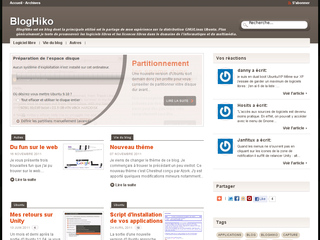
\includegraphics[width=0.5\textwidth]{./images/bloghiko.jpg}
    \caption{BlogHiko | 50\% de la largeur de la page}
\end{figure}
\section {Apport des enseignements dans le développement de la solution}
\section { compétences acquisent}
\section[Aide apportéé de par mes connaissances universitaires}


